\section*{Lucrarea de laborator \#2}
\phantomsection

\section{Scopul lucrarii de laborator}
Realizarea unui simplu Web Site personal
Realizarea unui mockup corespunzatorul site-ului care urmeaza a fi realizat
Familiarizarea cu HTML si CSS

\section{Mersul lucrarii de laborator}
\tab Pe parcursul lucrarii am efectuat un site si am unit cu el o baza de date.
Baza de date contine imagini si sunt adaugate dinamic pe site. Am creat patru
categorii de imagini care pot fi modificate de administrator. Totodata
administratorul poate adauga noi fotografii.\\
\tab Drept limbaj de programare pentru back-end am utilizat \textbf{Python}
Pentru front-end am utilizat \textbf{HTML/CSS}. Am utilizat frameworkul
\textbf{Django} si ca IDE am folosit \textbf{PyCharm}

\section{Screenshoturi din procesul de creare}
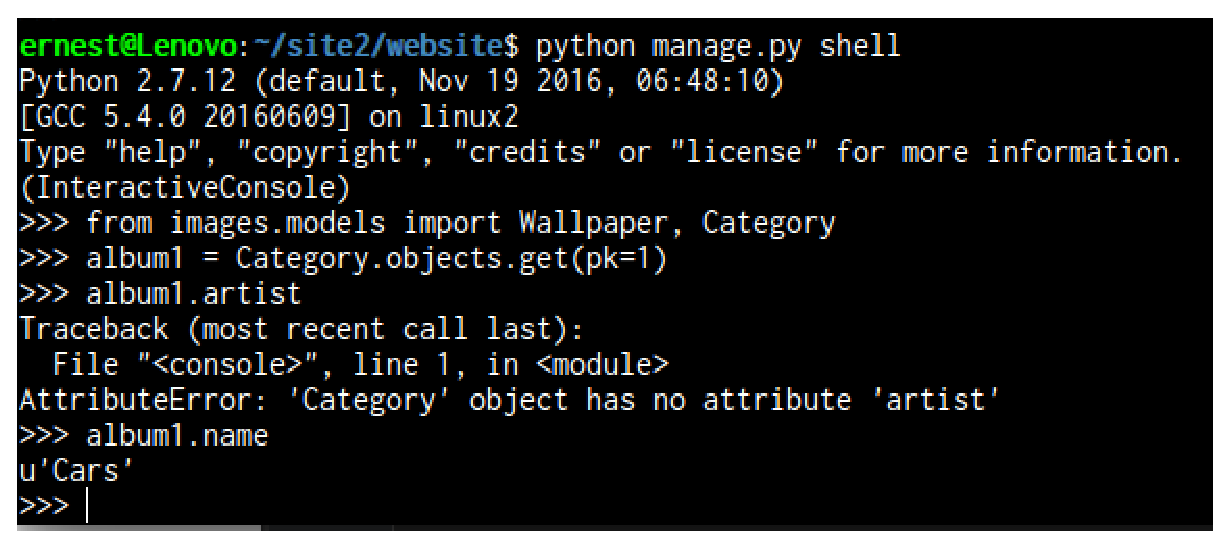
\includegraphics[width=\textwidth]{1.eps}
~\\
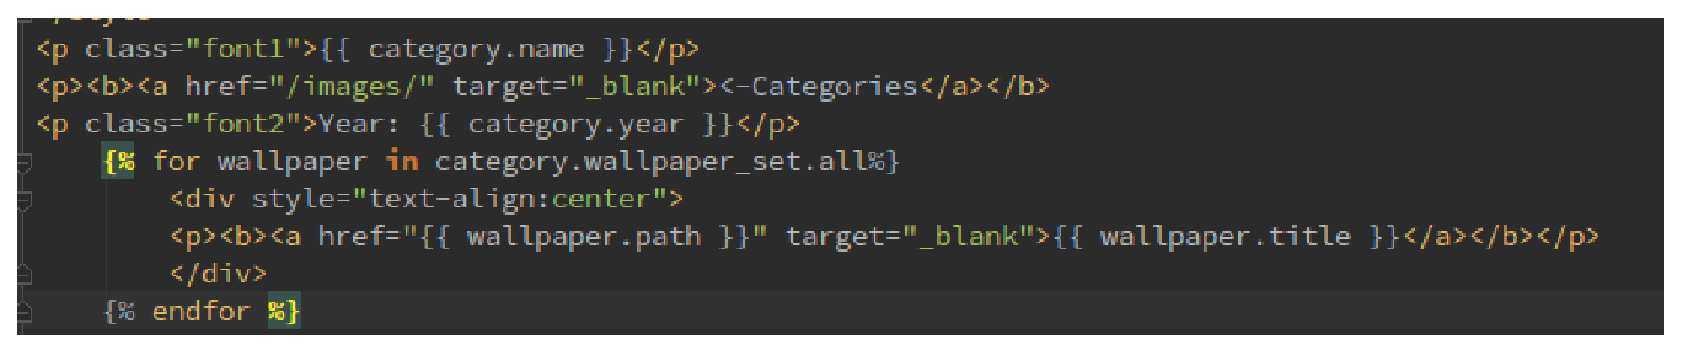
\includegraphics[width=\textwidth]{2.eps}
~\\
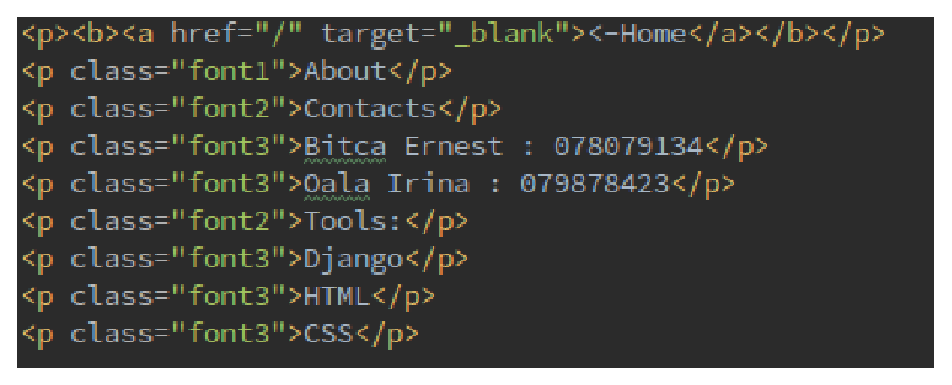
\includegraphics[width=\textwidth]{3.eps}
~\\
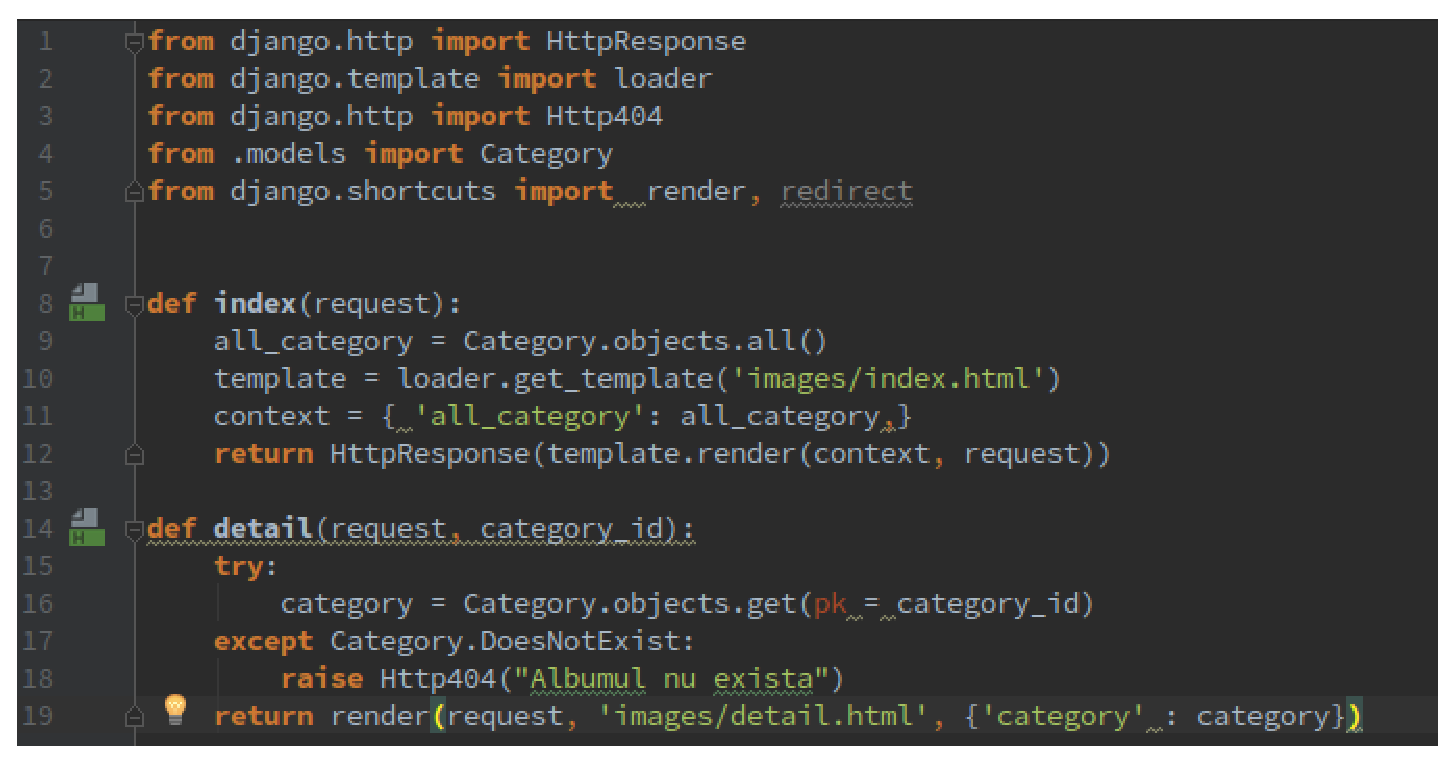
\includegraphics[width=\textwidth]{4.eps}
\clearpage
\section{Site Screenshots}

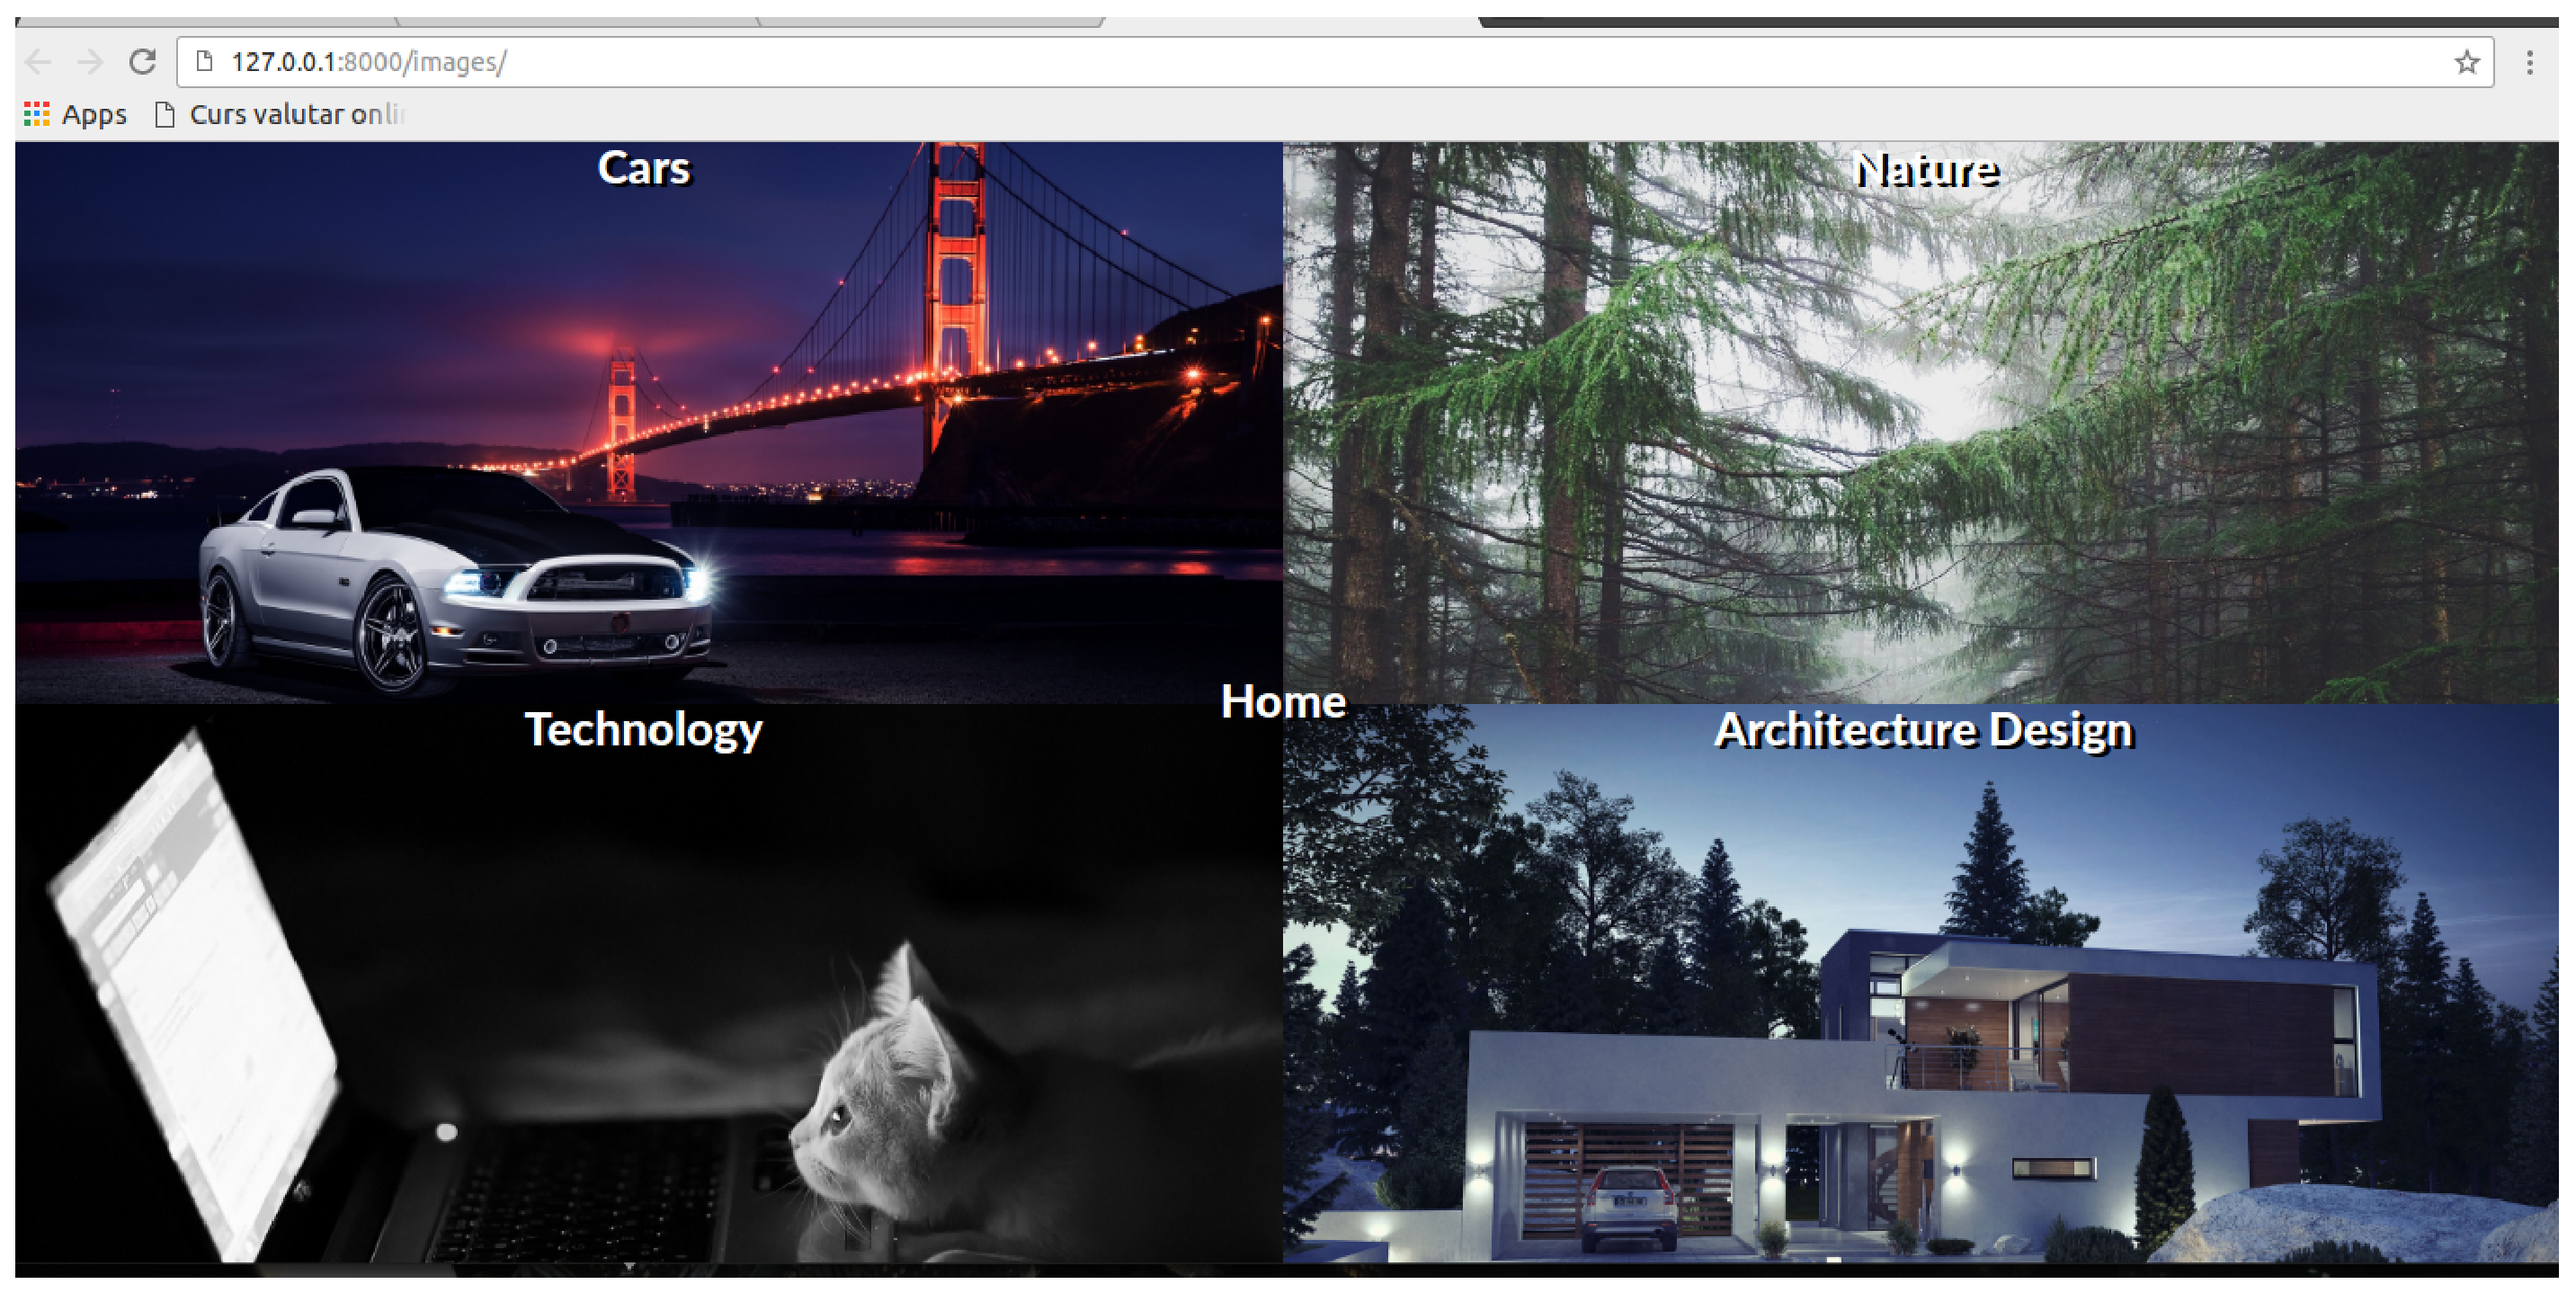
\includegraphics[width=\textwidth]{5.eps}
~\\
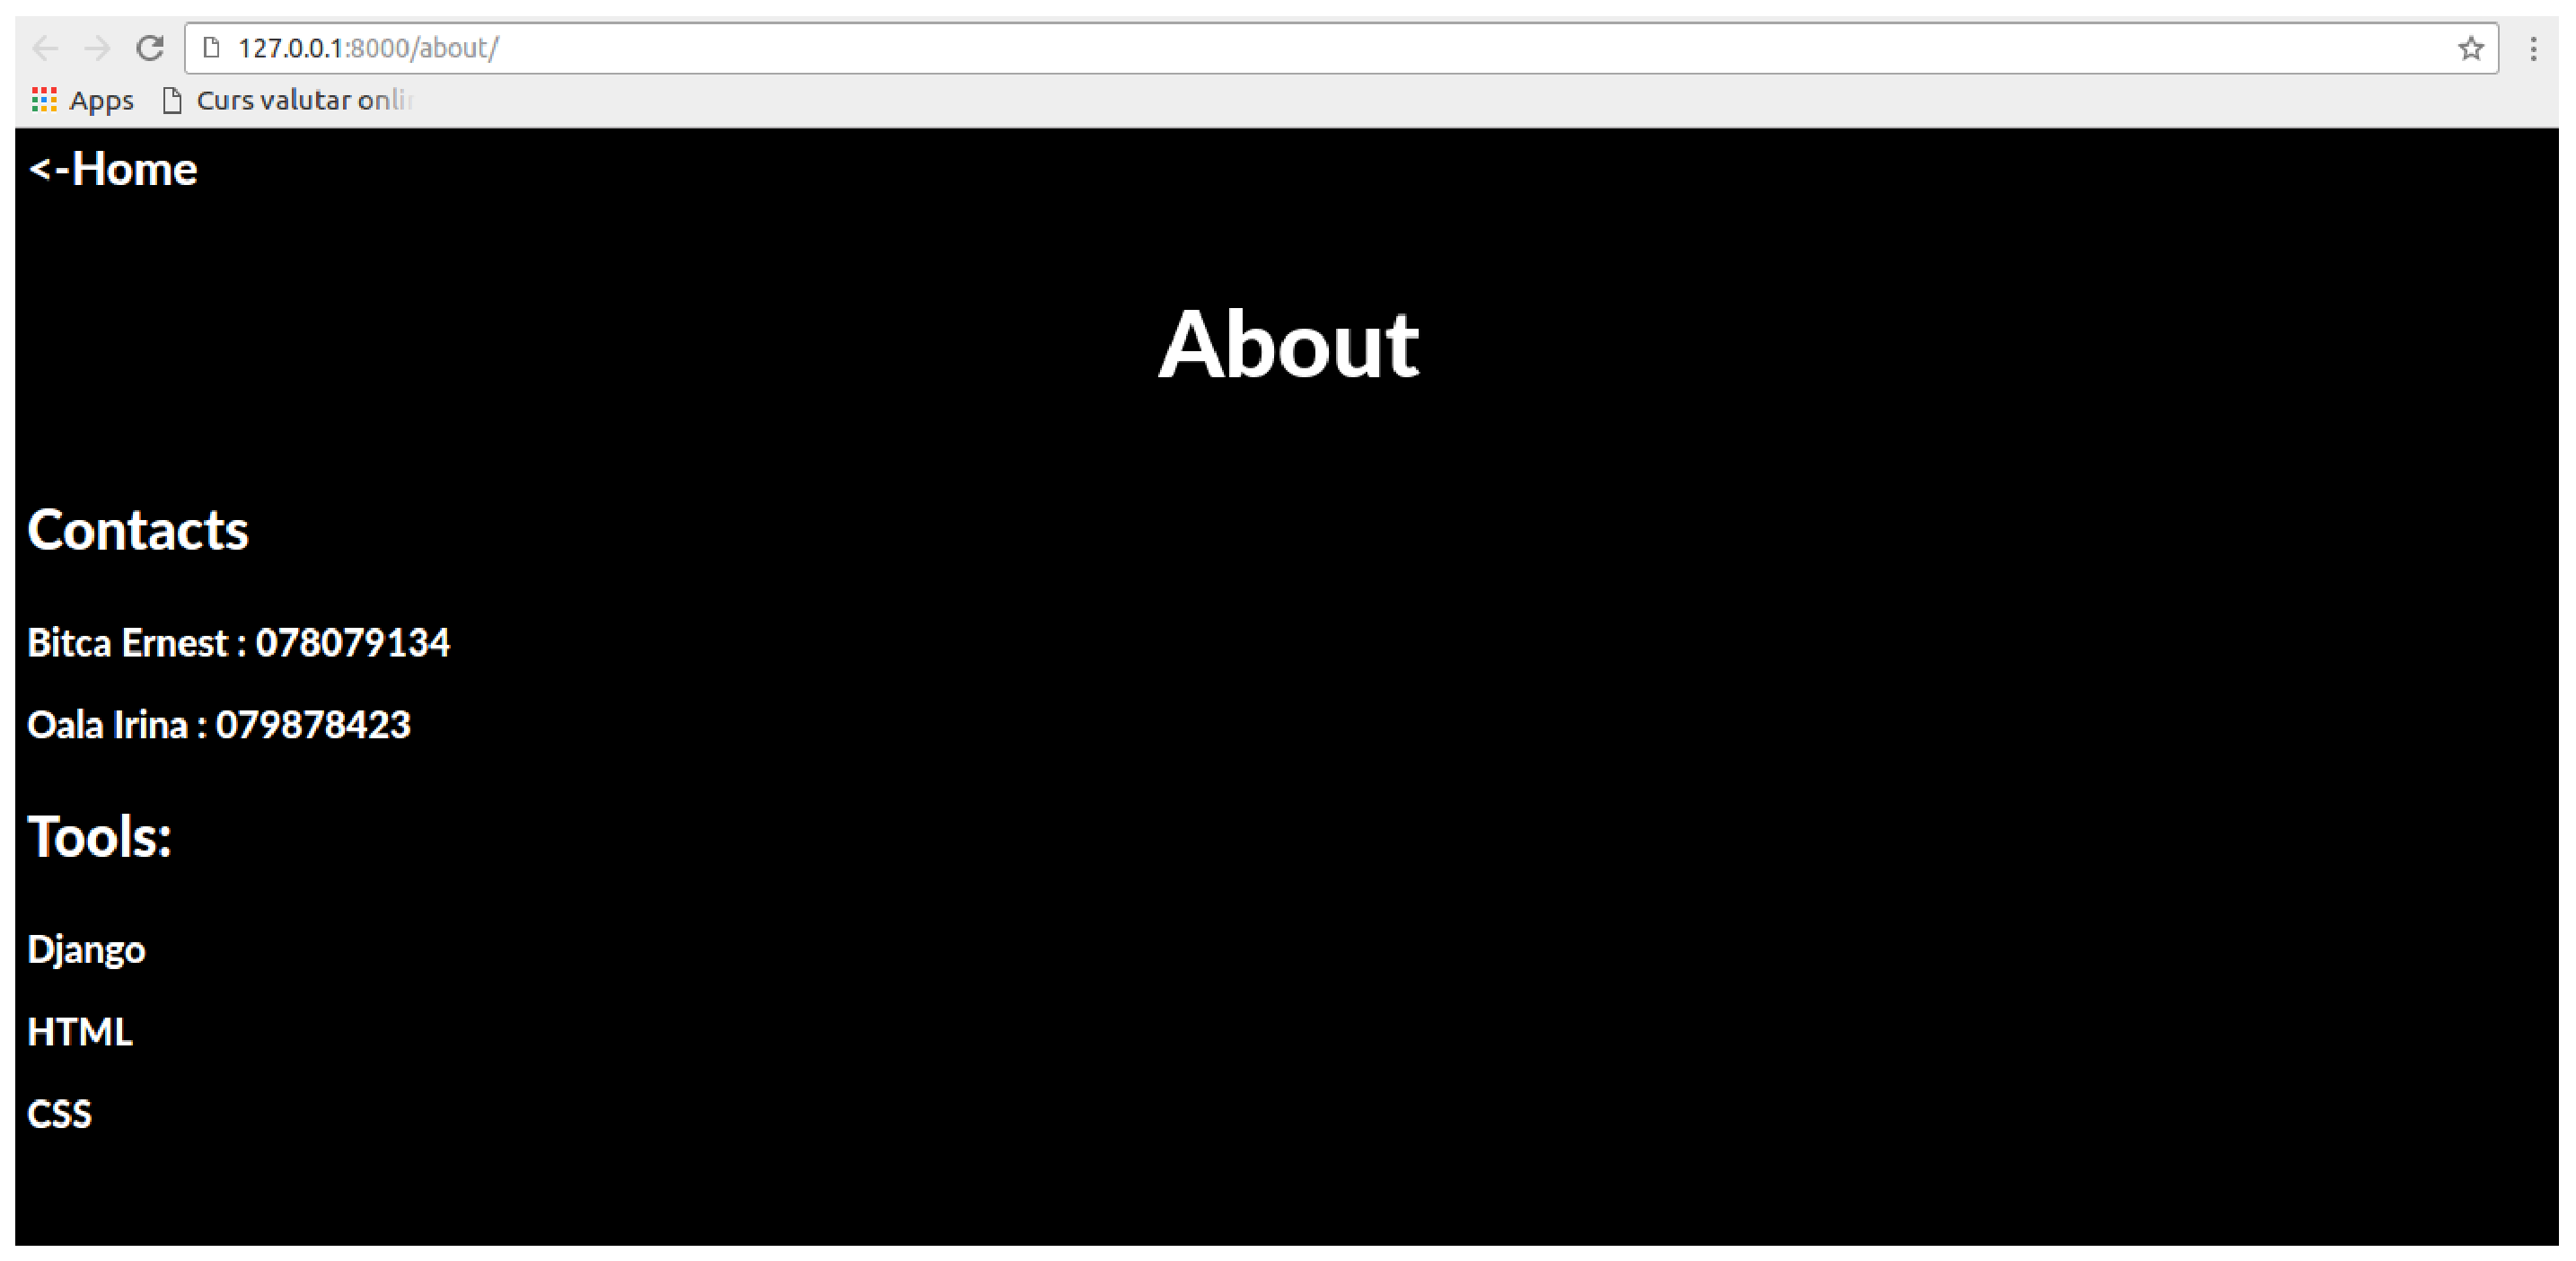
\includegraphics[width=\textwidth]{6.eps}

